\documentclass[hyperref, UTF8, 12pt]{article}
\usepackage{amssymb,amsfonts,amsmath,amsthm,latexsym}
\usepackage{subfigure}
\usepackage{float}
\usepackage{graphicx}
%\usepackage{fontspec,xltxtra,xunicode}
%\usepackage{times}

%----------
% 定义中文环境
%----------

\usepackage{xeCJK}

\setCJKmainfont[BoldFont={SimHei},ItalicFont={KaiTi}]{SimSun}
\setCJKsansfont{SimHei}
\setCJKfamilyfont{zhsong}{SimSun}
\setCJKfamilyfont{zhhei}{SimHei}
\setCJKfamilyfont{zhkai}{KaiTi}
\setCJKfamilyfont{zhfs}{FangSong}
\setCJKfamilyfont{zhli}{LiSu}
\setCJKfamilyfont{zhyou}{YouYuan}

\newcommand*{\songti}{\CJKfamily{zhsong}} % 宋体
\newcommand*{\heiti}{\CJKfamily{zhhei}}   % 黑体
\newcommand*{\kaiti}{\CJKfamily{zhkai}}  % 楷体
\newcommand*{\fangsong}{\CJKfamily{zhfs}} % 仿宋
\newcommand*{\lishu}{\CJKfamily{zhli}}    % 隶书
\newcommand*{\yuanti}{\CJKfamily{zhyou}} % 圆体

%----------
% 版面设置
%----------
%首段缩进
\usepackage{indentfirst}
\setlength{\parindent}{2em}

%行距
\renewcommand{\baselinestretch}{1.4} % 1.4倍行距

%页边距
\usepackage[a4paper]{geometry}
\geometry{verbose,
  tmargin=2cm,% 上边距
  bmargin=2cm,% 下边距
  lmargin=3cm,% 左边距
  rmargin=3cm % 右边距
}


%----------
% 其他宏包
%----------
%图形相关
\usepackage[x11names]{xcolor} % must before tikz,x11names defines RoyalBlue3
\usepackage{graphicx}
\usepackage{pstricks,pst-plot,pst-eps}
\usepackage{subfig}
\def\pgfsysdriver{pgfsys-dvipdfmx.def} % put before tikz
\usepackage{tikz}

%原文照排
\usepackage{verbatim}

%网址
\usepackage{url}

%----------
% 习题与解答环境
%----------
%习题环境
\theoremstyle{definition} 
\newtheorem{exs}{习题}

%解答环境
\ifx\proof\undefined\
\newenvironment{proof}[1][\protect\proofname]{\par
\normalfont\topsep6\p@\@plus6\p@\relax
\trivlist
\itemindent\parindent
\item[\hskip\labelsep
\scshape
#1]\ignorespaces
}{%
\endtrivlist\@endpefalse
}
\fi

\renewcommand{\proofname}{\it{证明}}

%==========
% 正文部分
%==========

\begin{document}

\title{基于卷积神经网络的图像分类系统}
\author{SJTU}
%\date{} % 若不需要自动插入日期,则去掉前面的注释;{ } 中也可以自定义日期格式
\maketitle

\section{任务介绍}
CIFAR-10 数据集由60000张图片组成,每张图片的大小为32 $\times$ 32,RGB三通道。整个数据集都被标记为十个标签的一种。数据集在下载后已经被分为5个训练Batch和1个测试Batch。每个Batch都包含10000张图片。\cite{krizhevsky2009learning}

\subsection{工作概述}
此Project进行CIFAR-10数据集的图像分类,需要基于CNN。由于数据集已经进行打包,我们直接使用数据集的训练集-测试集分类方法。我们完成的工作包括数据预处理,设计模型,设计训练策略,实际训练,进行训练总结(以文字和可视化的形式)。模型使用Pytorch工具,基于\url{https://pytorch.org/tutorials/beginner/blitz/cifar10_tutorial.html}. \\
\indent
在没有使用额外数据以及预训练模型的前提下,我们设计的模型准确率最高达到了92\%, 参数大小为83MB. 此外,按照要求,随机数种子被设为2021,便于审阅我们的结果; 如果想复现我们的结果,请参阅README.md.

\subsection {相关工作}
在\url{https://paperswithcode.com/sota/image-classification-on-cifar-10} 中含有使用此数据集模型排名。主流模型包括Transformer\cite{dosovitskiy2021image},ResNet\cite{kolesnikov2020big},EfficientNet\cite{tan2021efficientnetv2},DCN\cite{sousa2021cnn},ResNeXt\cite{Li_2019_CVPR}等。\\
\indent 从2012年有记录以来,年度最佳模型的准确率从88.8\%提高到了99.5\%。发表于2021CVPR的ViT-H/14将准确率提高到了99.5\%\cite{dosovitskiy2021image},而使用CNN的FlexConv在达到92.2\%以上准确率的同时\cite{romero2021flexconv},保证了自己的参数大小约为0.67MB,约为准确率最高的模型的$\frac{1}{1000}$.


\section{数据处理}
我们采取了以下数据预处理方式:
\begin{itemize}
\item 随机裁剪(Random Crop)
\item 随机水平翻转(Random Horizontal Flip)
\item 随机仿射变换(Random Affine)
\item 颜色抖动(Color Jitter)
\end{itemize}

\begin{figure}[H]
	\centering
	\subfigure[原始数据集]{
		\centering
		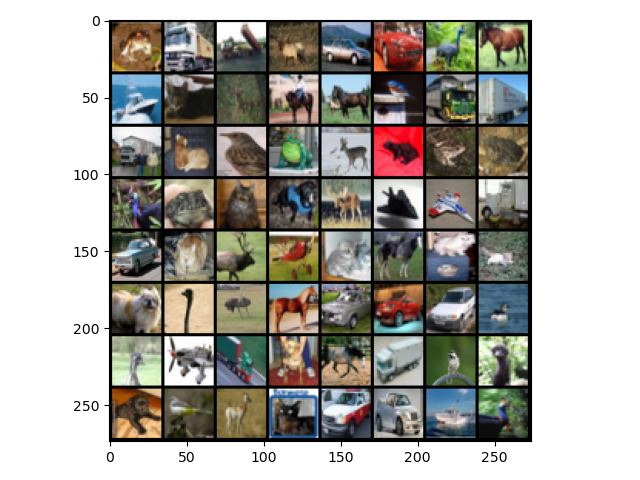
\includegraphics[width=0.4\linewidth]{original_dataset}
	}
	\subfigure[扩充数据集1]{
		\centering
		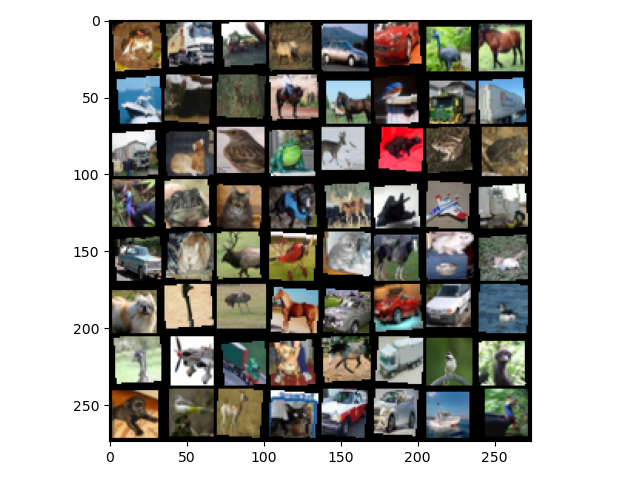
\includegraphics[width=0.4\linewidth]{augment1}
	}
	\subfigure[扩充数据集2]{
		\centering
		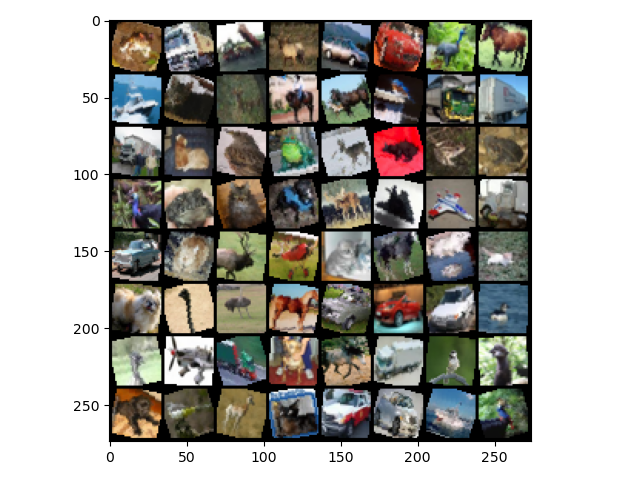
\includegraphics[width=0.4\linewidth]{augment2}
	}
	\subfigure[扩充数据集3]{
		\centering
		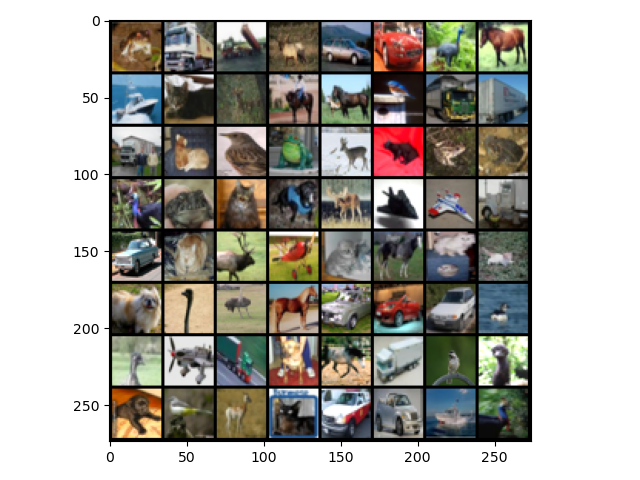
\includegraphics[width=0.4\linewidth]{augment3}
	}
	\caption{原始数据集,扩充数据集1(随机裁剪+随机水平翻转+随机仿射变换),扩充数据集2(随机放射变换),扩充数据集3(颜色抖动)}
\end{figure}
通过图像增强,我们扩充了数据集,为训练提供了更多样本。
\section{系统设计}
\subsection{架构选择}
\subsubsection{ResNet}
ResNet是时下应用最广泛的基于CNN的图像分类模型。\cite{he2015deep} 他的提出让CNN的层数由原来的不到十层提高到了上百层甚至上千层。原先人们发现随着CNN层数的增多,模型准确度反而下降。而这不能用过拟合来解释(因为训练集和测试集的Loss都同步上升),而随着BN大部分解决了梯度消失/爆炸问题后,模型退化问题仍然存在。这表明这可能时CNN架构本身的问题带来的。
\\ 
\indent
为了解决这个问题,ResNet提出了Shortcut方法,引入了恒等映射,让模型拥有了“什么都不做”的选择,有效防止了更多的层数带来的信息丢失。而更多的层数为分层学习提供了可能,每一层学到更细化的特征,提高了模型的表达能力;从而提高了模型的准确度。
\\ 
\indent
因此,我们的模型是基于ResNet的基本框架进行调参的。在ResNet论文\cite{he2015deep}中提出了5种ResNet模型,即ResNet18,ResNet34,ResNet50,ResNet101,ResNet152. 数字代表的是层数,我们尝试复现了以下框架。\ref{Fig.resnet1}
%% 一张
\begin{figure}[h] %H为当前位置,!htb为忽略美学标准,htbp为浮动图形
	\centering %图片居中
	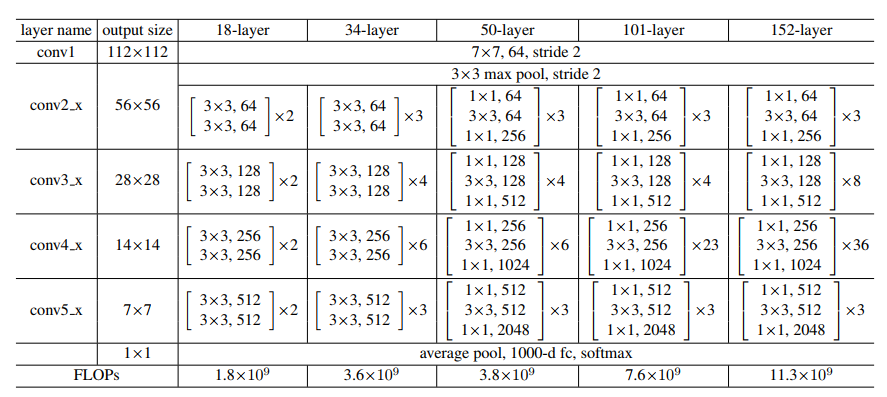
\includegraphics[width=0.7\textwidth]{resnet.png} %插入图片,[]中设置图片大小,{}中是图片文件名
	\caption{ResNet 论文中给出的模型结构} %最终文档中希望显示的图片标题
	\label{Fig.resnet1} %用于文内引用的标签
\end{figure}
\\
\indent
但是,在层数升至50层以上时,即使使用多块RTX3080 Ti显卡进行训练,也需要数小时甚至十余小时才能完成训练。我们优先将有限的资源使用在了低层数的ResNet上。特别对ResNet18(便于调参与快速训练查看结果)以及ResNet50(较好的平衡了层数和训练速度)进行了调参和训练。在最后,我们尝试进行了ResNet101的训练,事实证明,ResNet让模型层数更高,准确度也变得更好。
\\
\indent

\subsubsection{其他模型选择}
除了ResNet,我们还调研并且使用典型参数运行了一些在ResNet出现之前的较浅的CNN模型,包括vgg16,Inception10, alexnet8. 我们阅读了这些模型的Tensorflow实现并且试着本地运行了他们。您可以在Appendix A中审阅这些结果。我们发现无论Epochs小或者大,这些模型的训练结果都明显不如我们选择的ResNet. 因此,我们没有对这些模型进行进一步的调参和设计。

\subsection{ResNet架构说明}
上面提到了ResNet为新增加的层数引入了恒等映射的可能。我们希望能对$F(x) = H(x) - x$进行学习,因此学习到的原始特征应为$F(x) + x$. 这样残差为0时就时是恒等映射了。\\
\begin{figure}[h] %H为当前位置,!htb为忽略美学标准,htbp为浮动图形
	\centering %图片居中
	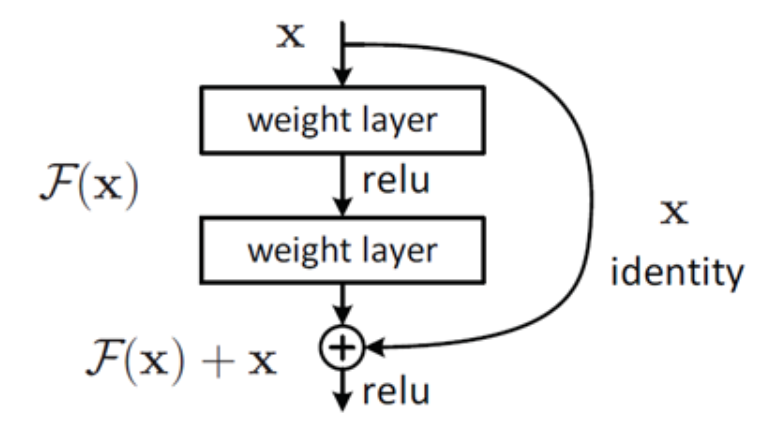
\includegraphics[width=0.5\textwidth]{resnetUnit.png} %插入图片,[]中设置图片大小,{}中是图片文件名
	\caption{ResNet 论文中的unit} %最终文档中希望显示的图片标题
	\label{Fig.resnet2} %用于文内引用的标签
\end{figure}
\indent
ResNet论文中提出了两种Residual Function. 分别应用于ResNet34-以及ResNet50+. 我们采用了这种模型设计。您可以在resnet\_all.py下面看到我们实现的两个残差单元~\ref{Fig.resnet4},分别命名为BasicBlock(left one)和BottleNeck(right one). 模型的全部架构都是由论文ImageNet架构指导~\ref{Fig.resnet1}对残差单元~\ref{Fig.resnet4}进行组装得到的。\\
\begin{figure}[h] %H为当前位置,!htb为忽略美学标准,htbp为浮动图形
	\centering %图片居中
	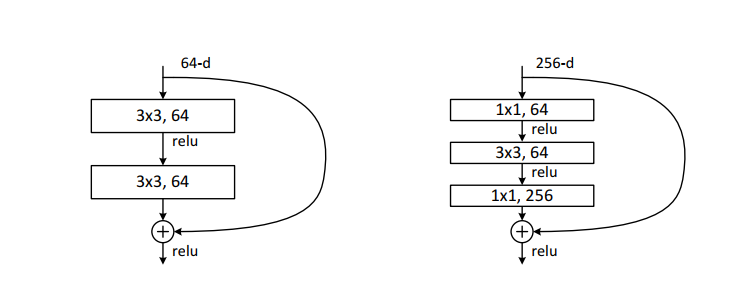
\includegraphics[width=0.95\textwidth]{resnet2units.png} %插入图片,[]中设置图片大小,{}中是图片文件名
	\caption{ResNet 论文中的两种Unit,我们在代码中分别进行了实现} %最终文档中希望显示的图片标题
	\label{Fig.resnet4} %用于文内引用的标签
\end{figure}
\indent
此外,我们将超参数抽离为变量,将数据预处理,模型调用和结果展示记录抽取出来,放在train.py中方便进行训练,实验和展示。您可以在上述两个代码文件中审阅我们的模型和训练计划。下图是结合了残差单元和架构说明对ResNet18的架构进行了更加清晰的展示。
\begin{figure}[h] %H为当前位置,!htb为忽略美学标准,htbp为浮动图形
	\centering %图片居中
	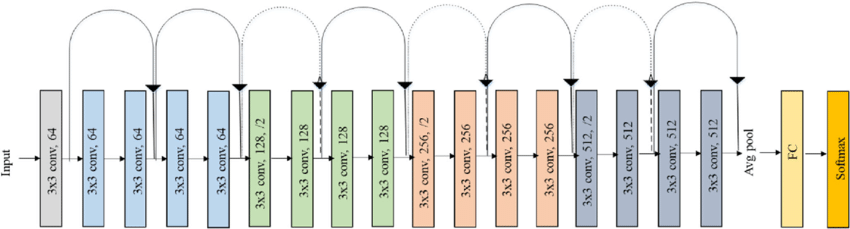
\includegraphics[width=0.95\textwidth]{resnet18.png} %插入图片,[]中设置图片大小,{}中是图片文件名
	\caption{ResNet18 展开} %最终文档中希望显示的图片标题
	\label{Fig.resnet3} %用于文内引用的标签
\end{figure}


\section{训练方法}
\subsection{选择调试超参数}
尽管我们尽可能提高了算力,但是限于ResNet的高层数, 我们的实验次数受到了限制,只能选择有限的超参数进行调试。ResNet论文\cite{he2015deep}为一些超参数提供了建议,比如Batch Size为128, lr为0.1.基于此,使用ResNet18架构,我们选择了以下参数进行调试:
\begin{itemize}
	\item Loss funtion: 损失函数指明了模型的训练目标, 我们对此进行了调研
	\item Epochs: Epochs过高可能导致过拟合,准确率下降。我们通过调研排除了这种可能
	\item Batch size: 每次翻倍调整Batch size直到计算资源不能支持
	\item Learning Rate: 从$10 ^ {-4}$跨数量级调试lr
	\item Learning Rate Decay: 对比pytorch中学习率调整方法
	\item Optimizer: 阅读论文筛选出了两个优化器进行比较, 同时调整优化器参数,包括weight decay 和momentum.
\end{itemize}

\subsection {损失函数}
尽管有人指出\cite{beyer2020imagenet}ResNet损失函数使用Binary Cross Entropy Loss的表现略好于Cross Entropy Loss,但我们并没有把重点放在损失函数的选取上。我们选择了多分类问题最常使用的Cross Entropy Loss函数。

\subsection{Epoch}
在模型超参数调试完成之后,我们发现每次Epoch在我们的训练集群上需要20S左右训练。考虑到训练和实验的总规模,我们把Epoch总数定为100和300两个MileStone. 100 Epochs达到时按要求记录报告准确率,200为最大迭代次数,时为了挖掘模型的最大准确率。我们阅读的论文有许多模型都会运行多达600个或者更多Epochs,限于算力,我们只运行200个并且保存测试集上工作的最好的参数报告。

\subsection{Batch size}
我们从8开始,依次调整Batch Size为8, 16, 64, 128, 256. 其中,Batch Size为256时,根据论文\cite{he2015deep} 建议,我们将learning rate 设置为了默认值的$110\%$. 由于显存限制,我们无法进一步提高Batch Size,否则训练速度可能会快速下降。实验完成后,我们选择最好的Batch Size进行下一步调试。

\subsection{Learning rate}
我们从$1 \times 10^{-4}$开始,依次提高Learning Rate为$1 \times 10^{-3}$, $1 \times 10^{-2}$, $1 \times 10^{-1}$, 观察Learning Rate在哪个数量级表现最好,并且能平衡模型收敛所需要的Epoch. 我们在这个数量级上进一步调试,直到选择一个比较好的Learning Rate进入下一步调参。

\subsection{Learning rate decay}
pytorch中主要支持6种学习率调整方法。一般而言,训练初期给予较大的学习率,随着训练进行,学习率逐渐减小能较好的平衡训练速度和准确率。在我们阅读的论文中,常使用的decay方法为StepLR(等间隔调整学习率,调整倍数为Gamma倍,调整间隔为step\_size epochs) 和 CosineAnnealingLR(以余弦函数为周期,在每个周期最大值时重新设置学习率). 在一篇基于ResNet讨论Warm restart的论文中\cite{loshchilov2017sgdr},作者建议使用后者进行学习率调整并且基于CIFAR10数据集做了实验。我们采用了他的实验结果,使用CosineAnnealingLR, warmup epochs 设为5.

\subsection{Optimizer and weight decay}
常见的优化器包括SGD, Adam, LAMB. 大部分的卷积神经网络都采用了SGD作为优化器,也有人采用Adam作为优化器,近几年的ResNet论文也有建议采用LAMB的。上述的Benchmark Top 1\cite{dosovitskiy2021image}论文中指出了在ResNet50模型中,各个优化器的表现是几乎没有差别的。\\
\indent
根据一个DL科学家的回答\cite{QuoraAnswer},使用SGD with momentum 更擅长于寻找"high-qualiyty and flat"的局部最小值,而Adam则更容易找到"sharp"的局部最小值。而前者带来了更好的泛化性和更低的性能损失,而且能够在其他超参数没有调试好的前提下带来还不错的结果。\\
\indent
我们同时尝试了SGD with momentum和 Adam, 其中前者的momentum 和weight\_decay 都采用了SGD优化器中的默认值,也即$momentum = 0.9, weight decay = 5 \times 10 ^ {-4}$;而Adam优化器的参数采纳了官方文档的推荐值,也即$lr = 1 \times 10^{-3}, \space betas=(0.9, 0.999), \space eps = 10 ^ {-8}, \space weight\_decay = 0$. (betas 为一阶和二阶的指数衰减率)我们对比了他们的效果,选择了相对更优秀的进行训练。

\section{实验与结果}
\subsection{平台}
使用了矩池云平台进行训练,租用了至多4块RTX3080 Ti显卡,CPU为8 $\times$ Xeon E5-2682 v4核心,86G内存。系统环境为Python3.7,CUDA 11.1,cuDNN 8.0.5,Pytorch 1.8.1, Horovod 0.22.1,Ubuntu 18.04.

\subsection{示例代码}
使用示例代码运行100 Epochs查看结果作为Baseline.

\subsection{超参数调试结果}
\subsubsection{Batch size}
\subsubsection{Learning rate}
\subsubsection{优化器}

\subsection{实验结果}
根据超参数调试结果,我们将基于准确率,训练时间,参数大小报告我们的实验结果。
\subsubsection{最终实验数据}
\begin{table}[h]
	\begin{tabular}{|l|l|l|l|l|l|}
		\hline
		Arch name & LR       & LR decay & Epochs   & Batch size & Warmup epochs \\ \hline
		Res18     & 4.20E+07 & cosine   & 1.68E+06 & 1.06E+06   & 5             \\ \hline
		Res50     & 8.55E+02 & cosine   & 3.42E+01 & 2.16E+01   & 5              \\ \hline
		Res101    & 1.17E+03 & cosine   & 2.93E+04 & 4.64E+04   &  5            \\ \hline
	\end{tabular}
\end{table}

\begin{table}[h]
	\begin{tabular}{|l|l|l|l|l|l|}
		\hline
		Arch name & Optimizer& Weight decay & Droupout   & Loss           \\ \hline
		Res18     & 4.20E+07 &         	    & No 	     & Cross Entropy  \\ \hline
		Res50     & 8.55E+02 &              & No         & Cross Entropy  \\ \hline
		Res101    & 1.17E+03 &              & No         & Cross Entropy  \\ \hline
	\end{tabular}
\end{table}

\begin{table}[h]
	\begin{tabular}{|l|l|l|l|l|l|}
		\hline
		Arch name & Running time & Hardware     & Param size     & Accuracy 	 \\ \hline
		Res18     & 4.20E+07     & 4.20E+07     & Cross Entropy  & 1897MB        \\ \hline
		Res50     & 8.55E+02     & 4.20E+07     & Cross Entropy  & LEVEL 8       \\ \hline
		Res101    & 1.17E+03     & 4.20E+07      & Cross Entropy &               \\ \hline
	\end{tabular}
\end{table}

\subsection{训练过程回顾}

\subsubsection{Tensorboard 数据}

\subsubsection{图示训练过程}

\section{Appendix A}
在选择方向的过程中,我们回顾了自从CNN提出以来的各种变体以及其成绩,并且获取了一些Tensorflow实现并且运行。您可以在./others里面查看这些模型并且复现结果。由于数据对显存要求远大于对显卡性能要求,我们没有保持硬件环境的一致。
\begin{table}[h]
	\begin{tabular}{|l|l|l|l|l|l|l|}
		\hline
		Arch name   & Hardware      & Param size & Epochs & Batch size & Running time & Accuracy \\ \hline
		VGG16       & Nvidia 2080Ti & 183.10 MB  & 100    & 32         & 61 mins      & 76.20\%  \\ \hline
		alexnet8    & Nvidia T80    & 115.67 MB  & 100    & 32         & 145 mins     & 61.62\%  \\ \hline
		resnet18-tf & Nvidia 2080Ti & 134.16 MB  & 100    & 32         & 59 mins     & 61.50\%    \\ \hline
		inception10 & Nvidia 2080Ti & 1.51 MB    & 100    & 32         &              &  73.66\%    \\ \hline
	\end{tabular}
\end{table}
\\
\indent
我们借此快速了解了各个模型的特点和能力,并且经过进一步了解,选择了ResNet继续研究。下图是这些模型的准确度,损失函数对于Epochs的图像:
\begin{figure}[H]
	\centering
	\subfigure[Alex8Net]{
		\centering
		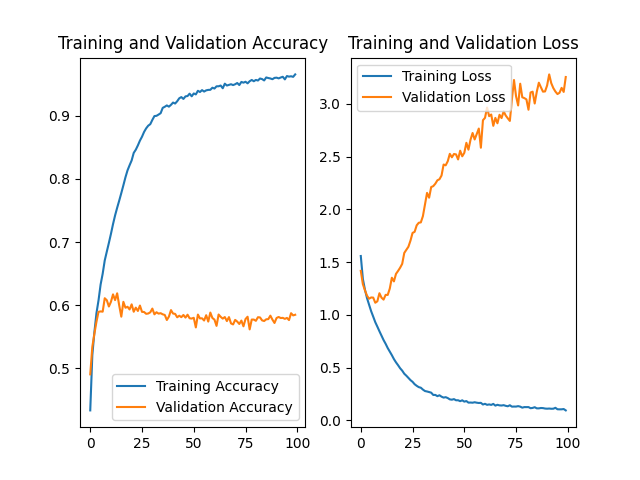
\includegraphics[width=0.4\linewidth]{alex8}
	}
	\subfigure[Vgg16]{
		\centering
		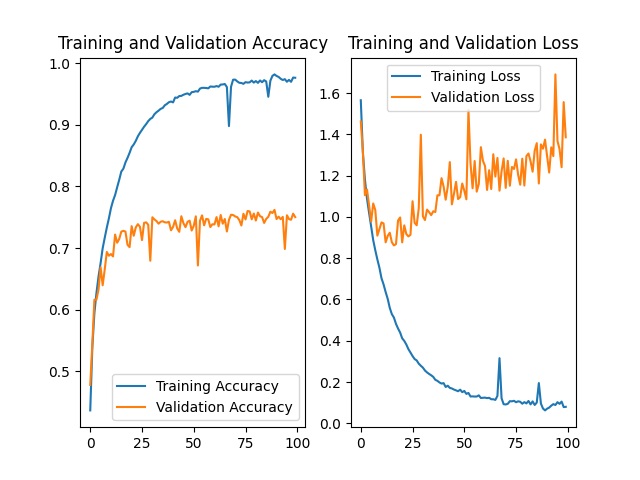
\includegraphics[width=0.4\linewidth]{vgg16}
	}
	\subfigure[Inception10]{
		\centering
		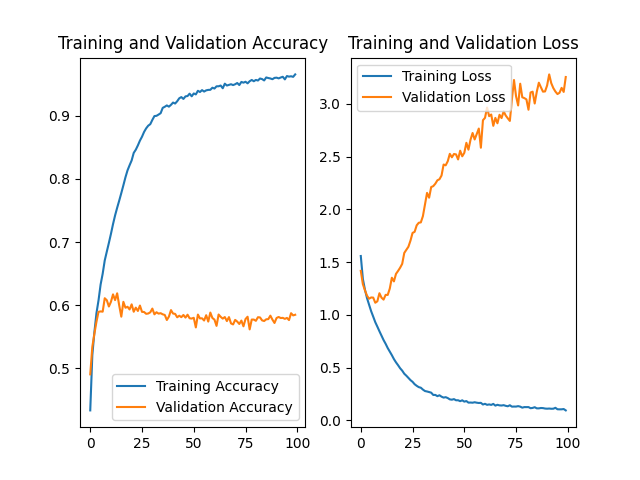
\includegraphics[width=0.4\linewidth]{inception10}
	}
	\subfigure[ResNet18]{
		\centering
		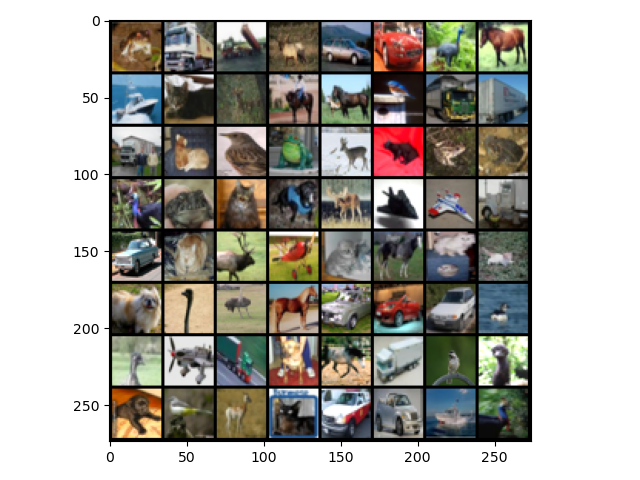
\includegraphics[width=0.4\linewidth]{augment3}
	}
	\caption{四种架构的朴素实现的实验结果}
\end{figure}

\section{模板介绍}
这个模板是UTF-8编码的,使用xeCJK宏包,中英文混排更美观,但编译速度稍慢。注意:该模板只能用xelatex编译。常用逻辑符号命令:
\begin{center}
\begin{tabular}{|c|c|c|}
\hline
名称      & 符号                   & 命令 \\
\hline
否定      & $\neg$                & \verb|\neg| \\
合取      & $\land$               & \verb|\land| \\
析取      & $\lor$                & \verb|\land| \\
蕴含      & $\to$                 & \verb|\to| \\
推出      & $\Rightarrow$         & \verb|\Rightarrow| \\
实质蕴涵   & $\supset$             & \verb|\supset| \\
双蕴含     & $\leftrightarrow$     & \verb|\leftrightarrow| \\
等价      & $\equiv$              & \verb|\equiv| \\
存在量词   & $\exists$             & \verb|\exists| \\
全称量词   & $\forall$             & \verb|\forall| \\
必然      & $\Box$                & \verb|\Box| \\
可能      & $\Diamond$            & \verb|\Diamond| \\
可满足,真  & $\models$            & \verb|\models| \\
语义后承   & $\vDash$,$\nvDash$   & \verb|\vDash,\nvDash| \\
句法后承   & $\vdash$,$\nvdash$   & \verb|\vdash,\nvdash| \\
属于      & $\in$,$\notin$       & \verb|\in,\notin| \\
真包含于   & $\subset$             & \verb|\subset| \\
包含于     & $\subset$            & \verb|\subset| \\
不等于     & $\neq$               & \verb|\neq| \\
小于等于   & $\leq$               & \verb|\leq| \\
大于等于   & $\geq$               & \verb|\geq| \\
下省略    & $\ldots$              & \verb|\ldots| \\
中省略    & $\cdots$              & \verb|\cdots| \\
对角省略  & $\ddots$              & \verb|\ddodts| \\
\hline 
\end{tabular}
\end{center}
更多符号对应的命令请参见:
\begin{itemize}
  \item \url{https://oeis.org/wiki/List_of_LaTeX_mathematical_symbols}或
  \item \url{https://www.ctan.org/tex-archive/info/symbols/comprehensive/}
\end{itemize}


\section{中文字体}

\subsection{字体切换}
默认字体为宋体。我们可以这样来改变中文字体:\heiti 从现在起是黑体。\kaiti 从现在起是楷体。\fangsong 从现在起是仿宋。\lishu 从现在起是隶书。\yuanti 从现在起是圆体。\songti 从现在起又是宋体。

\subsection{字体强调}
加粗字体自动变为黑体:\bf{粗体},加斜或强调字体自动变成楷体:\it{斜体},\emph{强调}。


\section{习题环境}

\begin{exs}
请证明勾股定理。
\end{exs}
\begin{proof}
这是证明。末尾后会自动添加方块以示结束。
\end{proof}

\begin{exs}
请计算 $1+2+\ldots +100$。
\end{exs}
\begin{proof}[解答]
这是解答。末尾后会自动添加方块以示结束。
\end{proof}

\nocite{*}
\bibliographystyle{acm}
\bibliography{ref.bib}
\end{document}
